\documentclass[a4paper,12pt]{article}
%%%%%%%%%%%%%%%%%%%%%%%%%%%%%%%%%%%%%%%%%%%%%%%%%%%%%%%%%%%%%%%%%%%%%%%%%%%%%%%%%%%%%%%%%%%%%%%%%%%%%%%%%%%%%%%%%%%%%%%%%%%%%%%%%%%%%%%%%%%%%%%%%%%%%%%%%%%%%%%%%%%%%%%%%%%%%%%%%%%%%%%%%%%%%%%%%%%%%%%%%%%%%%%%%%%%%%%%%%%%%%%%%%%%%%%%%%%%%%%%%%%%%%%%%%%%
\usepackage{eurosym}
\usepackage{vmargin}
\usepackage{amsmath}
\usepackage{fancyhdr}
\usepackage{listings}
\usepackage{framed}
\usepackage{graphics}
\usepackage{epsfig}
\usepackage{subfigure}
\usepackage{fancyhdr}

\setcounter{MaxMatrixCols}{10}
%TCIDATA{OutputFilter=LATEX.DLL}
%TCIDATA{Version=5.00.0.2570}
%TCIDATA{<META NAME="SaveForMode" CONTENT="1">}
%TCIDATA{LastRevised=Wednesday, February 23, 2011 13:24:34}
%TCIDATA{<META NAME="GraphicsSave" CONTENT="32">}
%TCIDATA{Language=American English}

\pagestyle{fancy}
\setmarginsrb{20mm}{0mm}{20mm}{25mm}{12mm}{11mm}{0mm}{11mm}
\lhead{Hibernia College} \rhead{Mr. Kevin O'Brien}
\chead{Mathematics for Computing}
%\input{tcilatex}

\begin{document}

% Question 1 - numbers - Started
% Question 2 - Sets - Not Started
% Question 3 - Logic - Not Started
% Question 4 - Functions - Started
% Question 5 - Graphs
% Question 6 - Digraphs and Relations
% Question 7 - 
% Question 8 -
% Question 9
% Question 10 - Matrices - STARTED

%---------------------------------------%
\subsection*{Question 1}
% 2003 Question 1
\begin{itemize}
\item[(a)] Working in base 2 perform the following calculation, showing all your working. [3 Marks]
\[110101_2 + 10111_2 - 100001_2\]
\item[(b)] Express the following hexadecimal number as a decimal number: $(A32.C)_{16}$.
[3 Marks]
\item[(c)] Convert the following decimal number into base 2, showing all your working:
$(253)_{10}$. \newline [2 Marks]
\item[(d)]  Express the recurring decimal $0.4242424\ldots$
 as a rational number in its simplest
form.\newline [2 Marks]
\end{itemize}
%---------------------------------------%
\subsection*{Question 2}
% 2002 Question 2
\begin{itemize}
\item[(a)] Let $S= \{w,x,y,z\}$. Describe briefly how the subsets of $S$ can each be represented by a unique 4-bit binary string. [2 Marks]
\item[(b)] Make a list of all 4-bit binary strings which have 1 as their first bit. Use this list to find all the subsets of $S$ containing the element $w$. [3 Marks]
\item[(c)] What is the total number of subsets of $S$? [1 Mark]
\item[(d)] Draw a Venn Diagram to show the three subsets A,B and C of a universal set $\mathcal{U}$
intersecting in the most general way. Shade the regions contained in the subset $X$ defined
by the membership table below. [2 Marks]\\ 
\begin{center}
\begin{tabular}{|ccc|c|}
  \hline
  % after \\: \hline or \cline{col1-col2} \cline{col3-col4} ...
  A & B & C & X \\\hline
  0 & 0 & 0 & 0 \\
  0 & 0 & 1 & 1 \\
  0 & 1 & 0 & 0 \\
  0 & 1 & 1 & 1 \\
  0 & 0 & 0 & 0 \\
  0 & 0 & 1 & 1 \\
  0 & 1 & 0 & 1 \\
  0 & 1 & 1 & 1 \\
  \hline
\end{tabular}
\end{center}
\item[(e)] Describe the subset X in terms of the sets A,B,C using the appropriate set operations. \newline [2 Marks]
\end{itemize}
\newpage
%---------------------------------------%
\subsection*{Question 3}
%2003 Question 4
\begin{itemize}
\item[(a)]

Let $n \in \{1,2,3,4,5,6,7, 8 ,9\}$ and let $p,q$ be the following propositions concerning the integer n.

\begin{itemize}
\item[p]: $n$ is even
\item[q]: $n < 5$.
\end{itemize}

Find the values of n for which each of the following compound statements is
true.
\begin{itemize}
\item[(i)] $\neg p$
\item[(ii)] $p \wedge q$
\item[(iii)] $\neg p \vee q$
\item[(iv)] $ p \otimes q$.
\end{itemize}

\item[(b)] Let p and q be propositions.
\begin{itemize}
\item[(i)]  Construct the truth table for $p \rightarrow q$. [2 Marks]
\item[(ii)] Use truth tables to prove that $\neg q \rightarrow \neg p$ = $p \rightarrow q$. [2 Marks]
\end{itemize}


\item[(c)] Let $p$, $q$ be the following propositions:
\begin{itemize}
\item[p] : this apple is red, 
\item[q] : this apple is ripe. 
\end{itemize}

Express the following statements in words as simply as you can. [2 Marks]
\begin{itemize}
\item[(i)] $p \rightarrow q$ \\
\item[(ii)] $p \wedge \neg q$.\\
\end{itemize}

\end{itemize}
\newpage

%---------------------------------------%
\subsection*{Question 4}
%2001 Question 4

\begin{itemize}
\item[(a)] A function $f$ is represented by the arrow diagram shown below.
\begin{center}
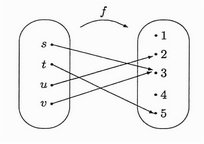
\includegraphics[scale=0.75]{HibCollArrow.jpg}
\end{center}

\begin{itemize}
\item[(i)] Give the domain, co-domain and range of $f$. [3 Marks]
\item[(ii)] Say why $f$ does not have the one-to-one property and why it does not
have the onto property, giving a specific counter-example in each case. [2 Marks]
\end{itemize}
\item[(b)]
\begin{itemize}
\item[(i)] State the conditions to be satisfied by a function $f : X \rightarrow Y$ for it to have
an inverse function $f^{-1} : Y \rightarrow X$. [3 Marks]
\item[(ii)] Define $f^{-1}$ when $X = \{1,2,3,4\}$, $Y = \{a,b,c,d\}$, and $f$ is given by the
table below. [2 Marks] \\
\begin{center}
\begin{tabular}{|c|cccc|}
  \hline
  % after \\: \hline or \cline{col1-col2} \cline{col3-col4} ...
  x & 1 & 2 & 3 & 4 \\ \hline
  f(x) & b & c & d & a \\
  \hline
\end{tabular}
\end{center}
\end{itemize}
\end{itemize}



%---------------------------------------%
\subsection*{Question 5}
%2002 Question 7
\begin{itemize}
\item[(a)] Let $\mathcal{S}$ be a set and let $\mathcal{R}$ be a relation on $\mathcal{S}$
Explain what it means to say that $\mathcal{R}$ is

\begin{itemize}
\item[(i)] reflexive
\item[(ii)] symmetrix
\item[(iii)] anti-symmetric
\item[(iv)] transitive [4 Marks]
\end{itemize}

\item[(b)]  Let $\mathcal{S}$ be the set $\{2,3,4,5,6,7\}$ and a relation $\mathcal{R}$ is defined between the elements of $\mathcal{S}$ by
    \begin{center}
\begin{quote}
x is related to y if $|x - y| \in \{0,3\}$.
\end{quote}
\end{center}
\begin{itemize}
\item[(i)] Draw the relationship digraph. [3 Marks]
\item[(ii)] Determine whether or not $\mathcal{R}$ is reflexive, symmetric or transitive. In cases
where one of these properties does not hold give an example to show that
it does not hold.n \newline [3 Marks]
\end{itemize}
\end{itemize}
\newpage

%---------------------------------------%
\subsection*{Question 7}
%2003 Question 7 - Good

\begin{itemize}
\item[(a)] A sequence is given by the recurrence relation
\[u_{n+1} = u_n + n \mbox{ and }u_1 = 0\]
\begin{itemize}
\item[(i)] Calculate $u_3$, $u_4$, and $u_5$. [2 Marks]
\item[(ii)] Use induction to prove the following [5 Marks]
\end{itemize}
\[u_n = \frac{n(n-1)}{2} \mbox{ for all n = 1} \]

\item[(b)] Write the following in $\sigma$ notation
\[ 1 + 4 + 7 + 10 + \ldots + (3n - 2)\]
Evaluate this when n = 100. [3 Marks]
\end{itemize}

%---------------------------------------%
\subsection*{Question 8}
% TREES
%2002 Question 7
\begin{itemize}

\item[(a)] What properties must a graph satisfy in order for it to be a tree? [2 Marks]
\item[(b)] Design a balanced binary search tree for an ordered list of 15 records.
Label the records $1,2, \ldots , 15$ in your tree. [4 Marks]

\item[(c)] A binary search tree is designed to store an ordered list of 50000 records,
numbered $1,2,3\ldots 50000$ at its internal nodes.
\begin{itemize}
\item[(i)] Draw levels 0, 1 and 2 of this tree, showing which number record is stored
at the root and at each of the nodes at level 1 and 2, making it clear
which records are at each level.
\item[(ii)] What is the maximum number of comparisons that would have to be
made in order to locate an existing record from the list of 50000? 
\end{itemize}
[4 Marks]
\end{itemize}


%---------------------------------------%
\subsection*{Question 10}
Consider the following matrices \textbf{A} and \textbf{B} which are given as


\[ A = \left(
  \begin{array}{ccc}
0 & 2 & 1 \\
2 &1 &2\\
1 &2 &0\\
  \end{array}
\right) \qquad
B = \left(
\begin{array}{ccc}
1 &0 &1\\
2 &1 &0\\
1 &2 &1\\
\end{array}
\right)
\]

\begin{itemize}
\item[(a)] Show that \textbf{AB} and \textbf{BA} are not equal. [3 Marks]
\item[(b)] Find matrices C, D and E such that
\begin{itemize}
\item[(i)] \textbf{B} + \textbf{C} = \textbf{A}
\item[(ii)] \textbf{BD} = \textbf{B}
\item[(iii)] \textbf{B} - \textbf{E} = \textbf{A}. [3 Marks]
\end{itemize}


\item[(c)]

\begin{itemize}
\item[(i)] Write down the augmented matrix for the following system of equations.
\item[(ii)] Use Gaussian elimination to solve the system. 
\end{itemize}
\[2x + y - z = 2\]
\[x - y + z = 4\]
\[x + 2y + 2z = 10\]
[4 Marks]
\end{itemize}
\end{document}
%--------------------------------------------%